\documentclass[pdf]{beamer}

\mode<presentation>{\usetheme{Warsaw}}
\usecolortheme{dove}

% http://web.mit.edu/rsi/www/pdfs/beamer-tutorial.pdf
% https://rohanverma.net/blog/2017/12/20/setting-up-latex-on-spacemacs/
% begin end CTRL-c CRTL-e

\AtBeginSection[]
{
  \begin{frame}
    \frametitle{Table of Contents}
    \tableofcontents[currentsection, hideothersubsections]
  \end{frame}
}

\usepackage[defaultfam,tabular,lining]{montserrat} %% Option 'defaultfam'
%% only if the base font of the document is to be sans serif
\usepackage[T1]{fontenc}
\renewcommand*\oldstylenums[1]{{\fontfamily{Montserrat-TOsF}\selectfont #1}}

\definecolor{ao(english)}{rgb}{0.0, 0.6, 0.0} % warning: duplicate below
\definecolor{azure(colorwheel)}{rgb}{0.0, 0.5, 1.0} % warning: duplicate below
\definecolor{darkgray}{rgb}{0.4, 0.4, 0.4}
\newcommand{\entity}[1]{\textcolor{ao(english)}{#1}}
\newcommand{\intent}[1]{\textcolor{azure(colorwheel)}{#1}}
\newcommand{\demo}[1]{\textit{\textcolor{darkgray}{#1}}}

\newcommand{\pgreen}[1]{\color<#1>[rgb]{0.0, 0.6. 0.0}}
\newcommand{\pblue}[1]{\color<#1>[rgb]{0.0, 0.6, 1.0}}

\title{Automatically responding to customers}
\begin{document}

\begin{frame}
  \titlepage
\end{frame}

\begin{frame}
  \frametitle{Table of Contents}
  \tableofcontents[hideothersubsections]
\end{frame}

\section{Introduction}
\subsection{Research question 1}
\begin{frame}{Existing benchmarks}
  \begin{itemize}
  \item Braun et al.
  \item Snips (next slide)
  \item Burtsev et al.
  \item Botfuel
  \end{itemize}
\end{frame}

\begin{frame}{Snips entity recognition}
  \begin{center}
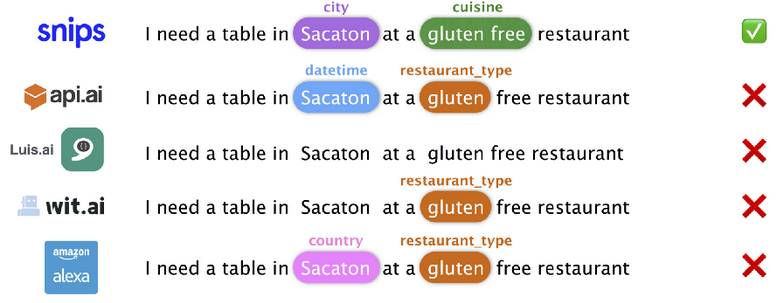
\includegraphics[width=\textwidth]{figures/snips_ner.png}
  \end{center}
\end{frame}

\begin{frame}{Results according to Snips}
  \begin{center}
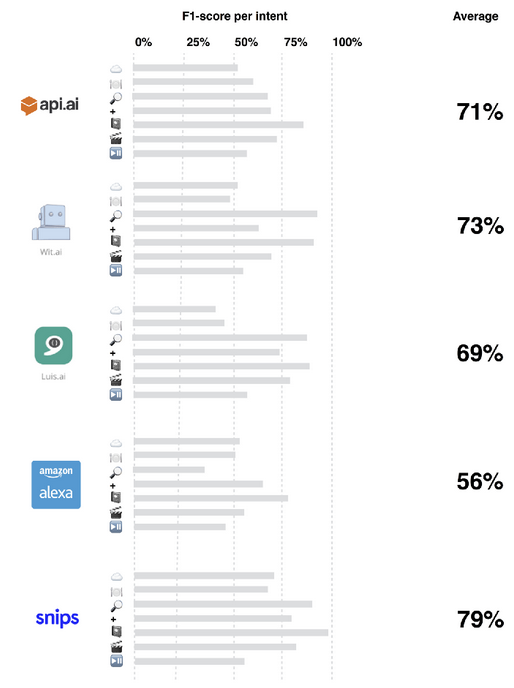
\includegraphics[height=0.85\textheight]{figures/snips_own_benchmark.png}
  \end{center}
\end{frame}

\begin{frame}{Question and goal}
  \begin{itemize}
  \item Can an open-source NLU benchmarking tool be created?
  \item Develop such a tool.
  \end{itemize}
\end{frame}

\subsection{Research question 2}
\begin{frame}{Improving accuracy}
 How hard can it be? 
\end{frame}

\begin{frame}{Question and goal}
  \begin{itemize}
  \item Can accuracy for NLU be increased?
  \item Improve the accuracy
  \end{itemize}
\end{frame}


\section{Preliminaries}
\subsection{Natural language processing}
\begin{frame}{Description of NLP field}
\begin{itemize}
\item Extract meaningful information from
  \begin{itemize}
  \item Text
    \item Speech
  \end{itemize}
\item Generate text
\end{itemize}
\end{frame}

\begin{frame}{Some well-known NLP tasks}
  \begin{itemize}
    \item Machine translation
    \item Speech recognition
    \item {\pgreen{2-3}{Named-entity recognition}}
    \item {\pblue{3}{Intent classification}}
    \end{itemize}
    \vspace*{5mm}
    \uncover<2-3>{\demo{What is [London's](\entity{location}) weather [tomorrow](\green{date})?}} \\[3mm]
    \uncover<3>{\demo{\intent{get\_weather}}}
\end{frame}
\begin{frame}{Language model}
  \begin{itemize}
    \item Rule-based
  \item Statistical
    \item Try to capture grammar
      \end{itemize}
      \vspace*{5mm}
      \uncover<2>{
  \begin{tabular}{l l}
        \textbf{Task} & \textbf{Example}\\
        \hline
        Spell correction & $P(\text{\demo{my car broke}}) > P(\text{\demo{my car boke}})$\\
        Machine translation & $P(\text{\demo{green house}}) > P(\text{\demo{house green}})$\\
        Speech recognition & $P(\text{\demo{the red car}}) > P(\text{\demo{she read ar}})$
  \end{tabular}
}
\end{frame}

\subsection{Deep learning}
{ % all template changes are local to this group.
    \setbeamertemplate{navigation symbols}{}
    \begin{frame}[plain]
       \hspace*{-6cm}
                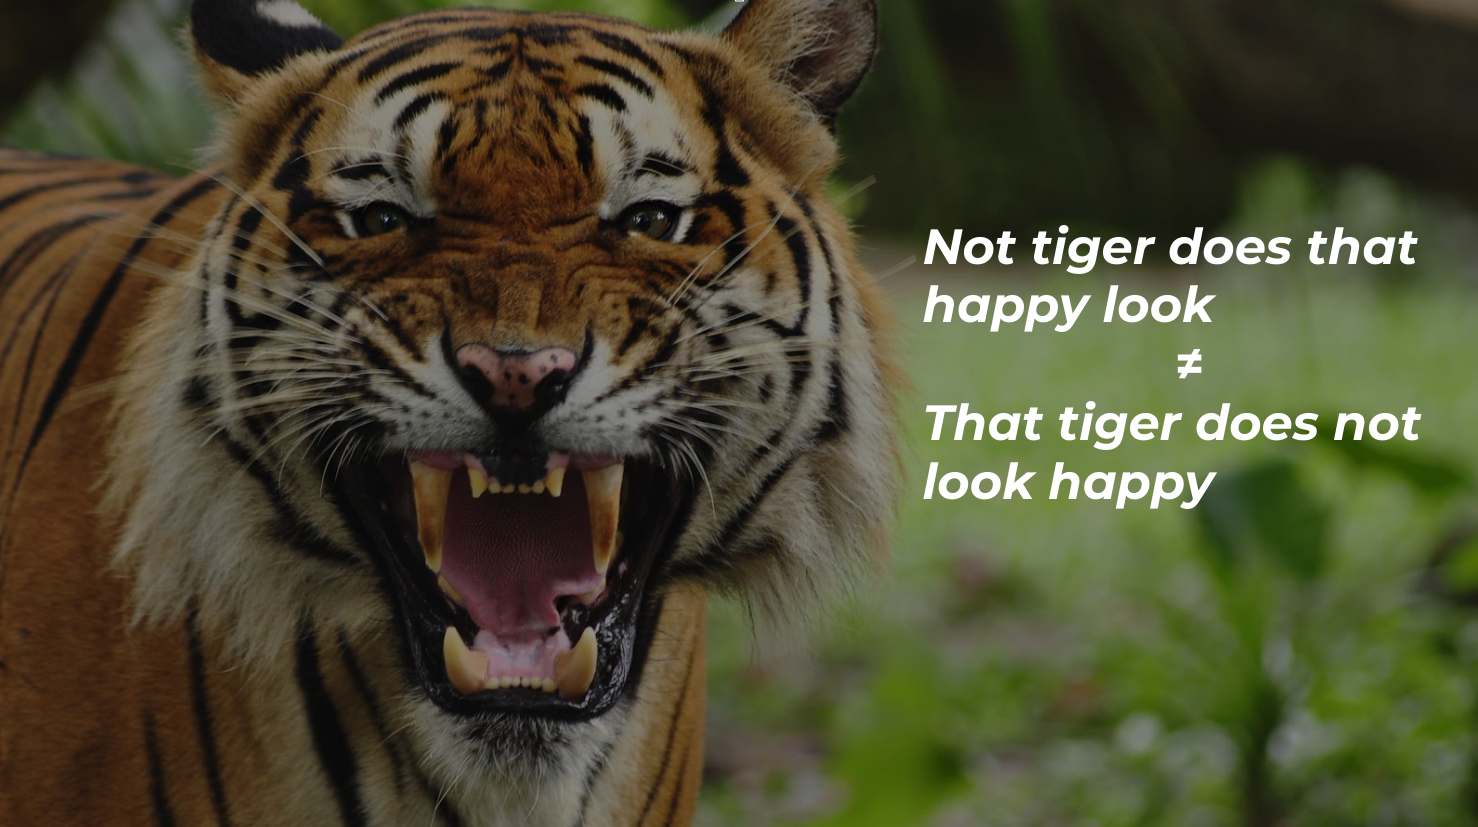
\includegraphics[scale=0.35]{figures/tiger.png}
     \end{frame}
}

\begin{frame}{Recurrent neural networks}
  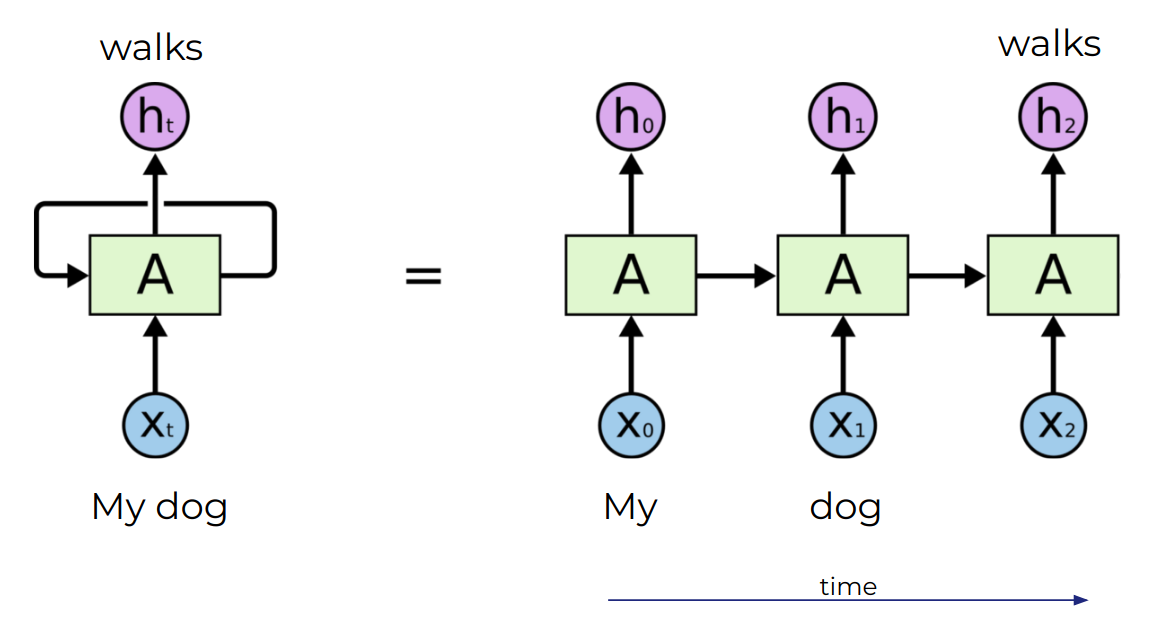
\includegraphics[width=\textwidth]{figures/rnn.png}
\end{frame}
  
\begin{frame}{Translating}
  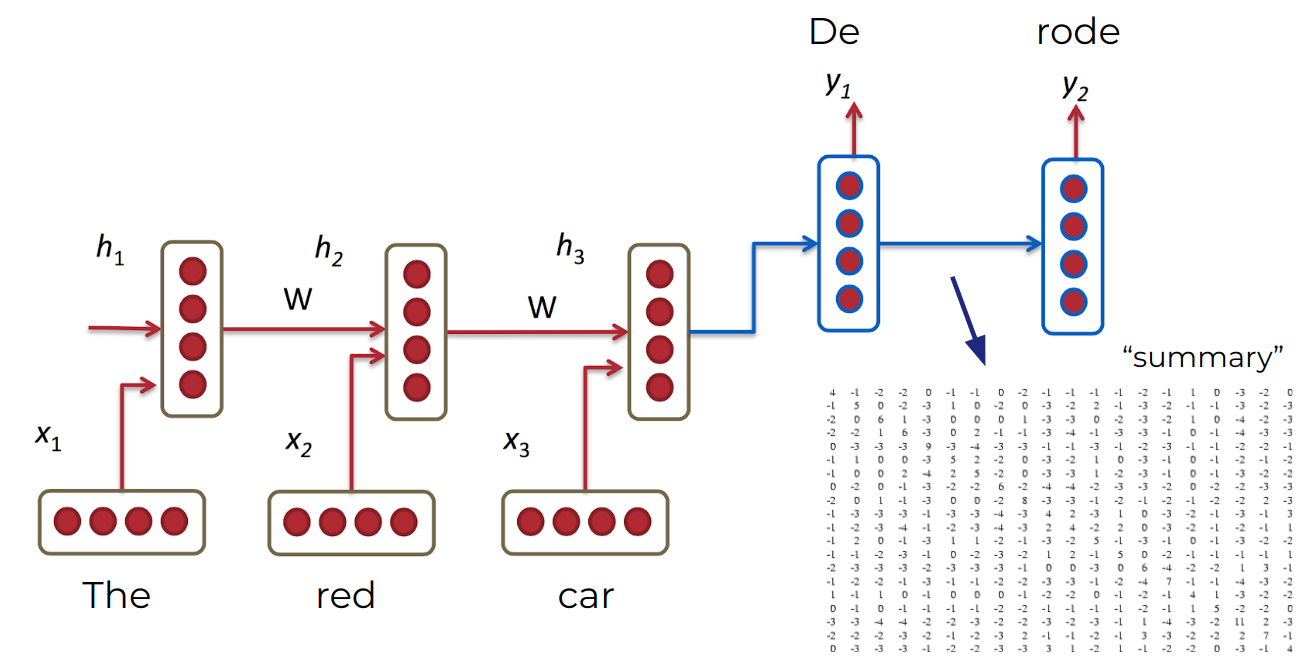
\includegraphics[width=\textwidth]{figures/encoder-decoder.png}
  \end{frame}

  \begin{frame}{Insufficient history}
    \begin{center}
      \demo{Norwegian \underline{frigate} sinking has far-reaching implications.}
      \end{center}
      \begin{center}
        \demo{Het zinken van het Noorse \underline{fregat} heeft verstrekkende gevolgen.}
      \end{center}
    \end{frame}

    \begin{frame}{Gated recurrent neural networks}
      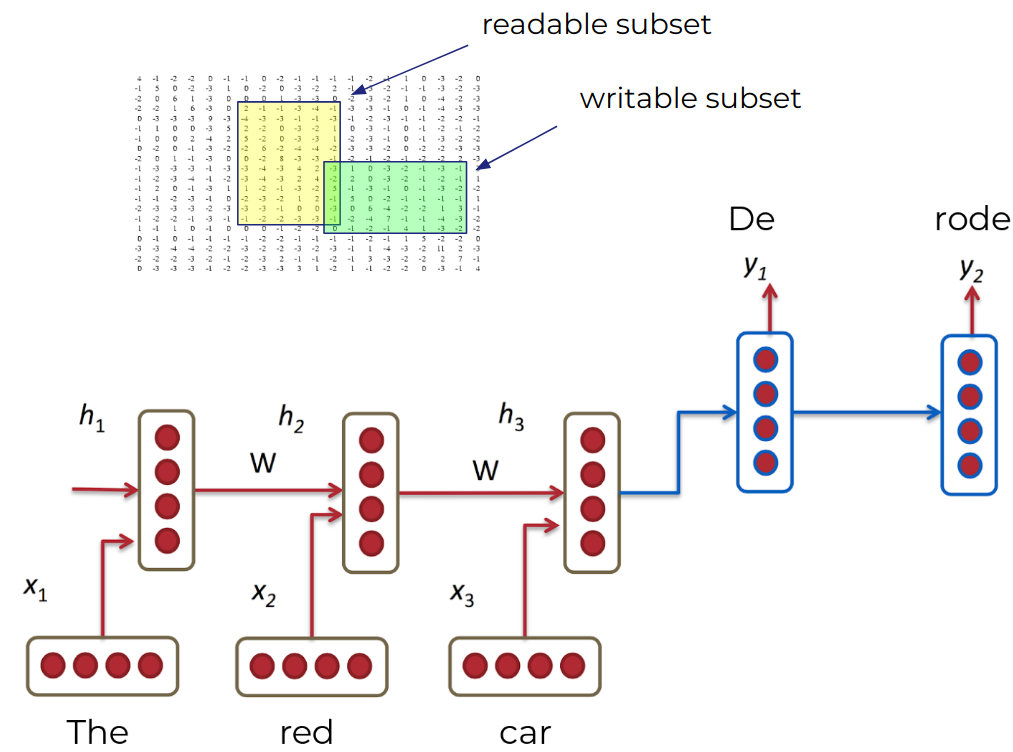
\includegraphics[height=0.9\textheight]{figures/gru.png}
      \end{frame}
    \section{Benchmarking}
\subsection{Datasets}
\begin{frame}{Overview}
   \begin{tabular}{l l l l l}
        \textbf{Dataset} & \textbf{Train} & \textbf{Test} & \textbf{\intent{Intents}} & \textbf{\entity{Entities}}\\
        \hline
        WebApplications & 30 & 54 & 7 & 1\\
        AskUbuntu & 53 & 109 & 4 & 3\\
        Chatbot & 100 & 106 & 2 & 5\\
        Snips2017 & 2100 & 700 & 7 & unknown\\
    \end{tabular}
  \end{frame}

  \begin{frame}{Example sentences}
    \begin{itemize}
    \item WebApplications\\ 
      \demo{How can I delete my [Hunch](\entity{WebService}) account?} \\
      \demo{\intent{DeleteAccount}}
    \item Chatbot \\
      \demo{when is the [next](\entity{criterion}) [train](\green{vehicle}) in
        [muncher freiheit](\entity{StationStart})?} \\
      \demo{\intent{DepartureTime}}
    \item Snips2017 \\
      \demo{i want to listen to [Say it Again](\entity{track}) by
        [Blackstratblues](\entity{artist})} \\
      \demo{\intent{PlayMusic}}
    \end{itemize}
    \end{frame}
\subsection{Systems}
\begin{frame}{Rasa}
  \begin{columns}
\column{0.5\textwidth}
\begin{itemize}
\item open-source
\item free
\end{itemize}
    \column{0.5\textwidth}
  \begin{center}
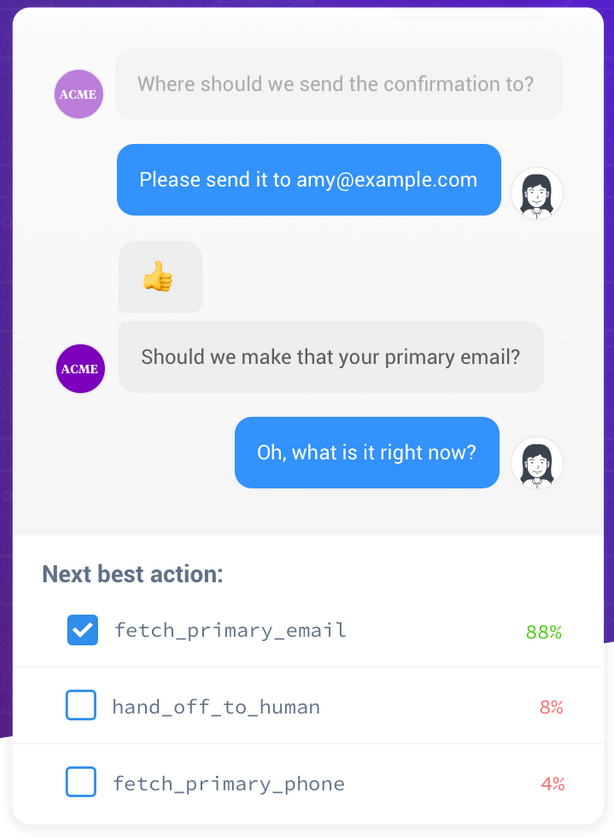
\includegraphics[height=0.9\textheight]{figures/rasa.png}
\end{center}
\end{columns}
  \end{frame}

  \begin{frame}{Cloud services}
\item  3
    \end{frame}
    
  \subsection{Results}

\section{Improving accuracy}

\section{Conclusions}
\subsection{Research question 1}
\begin{frame}{Research question 1}
\end{frame}

\subsection{Research question 2}
\begin{frame}{Research question 2}

\end{frame}
\end{document}
